
\chapter{Introduction}

\outline{
    The first chapter should introduce the problem studied and describe the main results obtained in the thesis.
    In order to provide guidance to the reader, the first chapter should briefly describe the organization of the rest of the thesis.
    The first chapter can also give the background of previous work on the subject and the method used in attacking the problem.
}

With the end of Dennard scaling, computer architects have sough to satisfy demand for increasing performance by providing specialized hardware accelerators tuned to computation with particular characteristics.
Perhaps the most successful examples of this trend is the uniform adoption and IEEE 754 specification of floating-point hardware, and widespread adoption of graphics processing units (GPUs) for more general data-parallel compute tasks.
With the success of GPUs as a template, architects are moving forward with a wide variety of specialized processors, such as
SIMD extensions~\todo{cite NEON, SSE, AVX},
AI accelerators~\todo{google tpu, huawei neural processing unit, ibm neuromorphic},
motion coprocessors~\todo{cite apple},
field-programmable gate arrays (FPGAs)~\todo{cite Intel, Xilinx}
network processors~\todo{cite intel ixp, netronome},
digital signal processors~\todo{cite google pixel2},
vision processing units~\todo{cite movidius, microsoft, mobilieye, MIT},
and many others.

\outline{memory wall}

The degree to which these accelerators are integrated with the host system varies.
Figure~\ref{fig:integration-spectrum} depicts how integrated some common accelerators are.
Fully-integrated accelerators are characterized by direct and transparent access to system memory, no additional programming system or compiler support, and no explicit control through an OS or vendor API.
For example, floating-point accelerators are fully integrated.
They have migrated into the host instruction-set architecture, have first-class access to system memory, and are supported without specialized toolchains or programming systems.
Similarly, SIMD vector extensions are nearly as integrated, but may require some special attention to memory alignment, precision, or rounding modes.
In contrast, fully-discrete accelerators have their own memory, have esoteric programming systems, and demand explicit control.
For example, FPGAs are programmed in hardware-description languages, may require the host system to be rebooted to be reconfigured, and often require the programmer to explicity transfer data to their memory.
As on the of the most mature accelerators, GPUs occupy a middle ground.
GPUs vary from partially-integrated to discrete: when a GPU is integrated on the same die as the CPU, it may share the same physical memory, but the computation model remains for compute tasks to be ``offloaded'' to the GPU, with the CPU managing the execution.

\begin{figure}
    \centering
    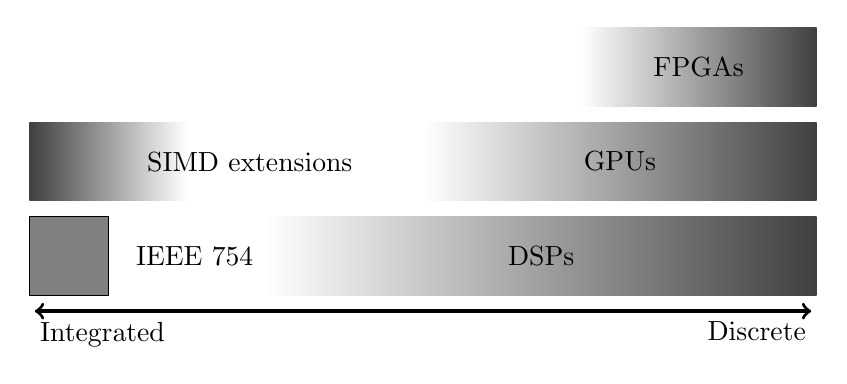
\begin{tikzpicture}[
        nodestyle/.style={},
        axisline/.style={
            <->,
            very thick,
            shorten <=2pt,
            shorten >=2pt,},
        axistext/.style={},
        ]

        \pgfmathsetmacro{\rt}{1} % thickness
        \pgfmathsetmacro{\rs}{0.2} % spacing

        \pgfmathsetmacro\ra{\rs}
        \pgfmathsetmacro\rb{\ra+\rt+\rs}
        \pgfmathsetmacro\rc{\rb+\rt+\rs}


        \draw[axisline] (0,0) node[anchor=north west] {Integrated} -- (10,0) node[anchor=north east] {Discrete};

        \draw[fill=gray] (0,\ra) rectangle (1,\ra+\rt);
        \node [above] at (2.1, \ra+0.25\rt) {IEEE 754};

        \shade[left color=darkgray, right color=white] (0,\rb) rectangle (2,\rb+\rt);
        \node [above] at (2.8, \rb+0.25\rt) {SIMD extensions};

        \shade[left color=white, right color=darkgray] (3,\ra) rectangle (10,\ra+\rt) node[pos=0.5] {DSPs};
        \shade[left color=white, right color=darkgray] (5,\rb) rectangle (10,\rb+\rt) node[pos=0.5] {GPUs};
        \shade[left color=white, right color=darkgray] (7,\rc) rectangle (10,\rc+\rt) node[pos=0.5] {FPGAs};

    \end{tikzpicture}
    \caption{Spectrum of integration for accelerators.}
    \label{fig:integration-spectrum}
\end{figure}

Thanks to \todo{fundamental physical challenges}, accelerators require memories close to their high-performance specialized compute elements.
Without these memories to ``feed the beast'', the performance of the accelerator would be severely limited by its link to the host memory.
For discrete-type accelerators, moving data into accelerator memory to support high-performance execution is a first-order developer challenge.
This work lays the foundation for mitigating the data-placement challenge and reducing developer effort.

\todo{cognitive computing apps as a motivating example}

The data-placement and data-movement challenge is exacerbated by the growing demand for data-driven applications.
Analytics and neural-network applications ingest huge amounts of data, and even if the amount of compute per data element is small, the aggregate required computation can be commensurately large.
That motivates developers to use accelerators for these applications.
To achieve high performance on accelerators, developers must marshal and coordinate their data movement and computation.

Any automated solution to this problem will require a detailed characterization of the underlying heterogeneous system and its data movement capabilities.
This work demonstrates a systematic heterogeneous system communication characterization.
Furthermore, it presents a systematic method for analyzing applications to determine how their performance is influenced by heterogeneous systems.

The rest of this document is organized as follows:
chapter 2 describes background and related work;
chapter 3 describes the hardware system characterization approach;
chapter 4 describes the application characterization approach;
chapter 5 describes the methodology for combining the system and application characterization to understand application performance;
chapter 6 discusses related work;
and finally, chapter 7 concludes.
